\documentclass[a4paper, 11pt, oneside]{book}
\usepackage[utf8]{inputenc}
\usepackage{setspace}
\usepackage{geometry}
\newgeometry{left=3.5cm,right=2.5cm,top=2.5cm,bottom=2.5cm}

\makeatletter
\newif\if@restonecol
\makeatother
\let\algorithm\relax
\let\endalgorithm\relax
\usepackage[linesnumbered,ruled,algonl,vlined]{algorithm2e}


\usepackage{graphicx}
\usepackage{epstopdf}
\DeclareGraphicsExtensions{.pdf,.eps,.png,.jpg,.mps}
\usepackage{placeins} % for \FloatbBarrier

\newtheorem{theorem}{Theorem}[section]
\newtheorem{corollary}{Corollary}[theorem]
\newtheorem{lemma}[theorem]{Lemma}

\renewcommand\floatpagefraction{.9}
\renewcommand\topfraction{.9}
\renewcommand\bottomfraction{.9}
\renewcommand\textfraction{.1}

\frenchspacing \sloppy


\newcommand{\eat}[1]{}
\hyphenation{}

\begin{document}

\title{Ensemble Learning in Data Streams}


\author{
Hossain Mahmud \\
Technische Universit\"at M\"unchen\\
mahmud@in.tum.de
}

\date{}

%\maketitle

%\normalsize
\onehalfspacing

\section{Related Works}
\label{chp:relworks}
Compared to data mining, stream mining is a young area. Most of the methods date back only a couple of decades. Similarly, the concept of ensemble learning was first introduced in the traditional batch learning, however, ensemble adaptations for streams are fairly new concepts. In this chapter, we list the most influential methods developed so far with particular focus on tree based learners. We follow a rudimentary narrating style starting directly with methods for general stream learners for stationary streams, and then for evolving data streams. After that, we list the base methods for ensemble learning, and finally we present ensemble based stream learners.

\subsection{Stream Mining}
%Compared to the classical data mining approaches stream mining is relatively a newer topic to be addressed in literature. Even though for batch approaches both classification and clustering problems have been vastly studied, their stream adaption remains a challenge due the restrictions imposed by the stream data. Possibility of temporal locality makes the classification problem harder in a streaming environment. Algorithms needs to address the evolution of underlying data stream. 

Domingos and Hulten introduced a strict one-pass adaptation of decision tree approach~\cite{breiman84:dt,quinlan93:c45} for data streams. Classic approaches like ID3 and C4.5 learners assume that all training examples can be stored in the main memory altogether. This is a significant limitation to the number of examples these algorithms can handle. Similarly, disk based decision tree learners (SLIQ~\cite{mehta96:sliq}, SPRINT~\cite{shafer96:sprint}, etc.) become very expensive when data sets are very large and the expected trees has many levels. Domingos and Hulten proposed \textit{Very Fast Decision Trees (VFDT)}~\cite{domingos00:vfdt} that uses the Hoeffding bound~\cite{hoeffding63:bound} to build an anytime decision tree for constant memory and time. The primary assumption in this approach is that to find the best attribute for a node in a decision tree, it may be sufficient to consider only a fraction of the training set that passes through that node. The Hoeffding bound provides a statistical measure to determine how much data is needed to ensure a level of degree of certainty, i.e. the error margin would be bounded by a given value~\cite{catlett91:thesis}.

Like most statistical and machine learning algorithms VFDT assumes that training data is randomly drawn from a stationary distribution. This assumption is not valid for large databases and data streams. Over time an underlying method or environment that generates data could change. The shift is  referred to as {\it concept drift} in the literature and can be abrupt as well as very slow. Data related to weather forecast, economic condition prediction, mis-calibrated sensors, etc. are examples of a concept drifting environment. A concept-adaptive variant of VFDT, \textit{CVFDT}~\cite{hulten01:cvfdt}, can handle such scenarios. CVFDT updates its decision rules, essentially the tree structure, by detecting the concept drift in the data. It maintains alternate subtrees whenever an old subtree becomes questionable, and replaces the old one with the alternative when it becomes more accurate. CVFDT uses a sliding window and updates sufficient statistics by increasing the count of newly arrived examples and decreasing the count of old examples in the window. Essentially CVFDT achieves same accuracy that would be achieved if VFDT had been run again with the new data. CVFDT does this in $O(1)$ time with an additional space requirement as compared to the VFDT's $O(w)$ complexity where $w$ is the window size. Another extension of VFDT, VFDTc was proposed in~\cite{gama05:vfdtc} that improves VFDT by handling continuous numeric attributes and adding na\"ive Bayes prediction at the leaves of the tree.


% TODO: briefly include multi-label evolving ...
% TODO: frequent item set mining]

\subsection{Ensemble Learning}
Traditional machine learning algorithms generally feature a single model or classifier such as \textit{na\"ive Bayes} or \textit{multilayer perceptron (MLP)}. The free parameters of these learners (e.g. weights of feed-forward neural network) are set by realizing the complete training set. These classifiers provide a measurement of the generalization performance i.e. how well the classifier generalizes the training set. However, given a finite set of training example, it is rather reasonable to assume that the data might contain several generalizations. For example, a different setting of the neural network classifier (weights, node layers, node counts, etc.) changes the final network to some extent. For stream environment, this assumption becomes trivial. Thus, choosing a single classifier is not always optimal. Using the best classifier among several classifiers where each is trained with the same training set would be an alternative, however, information is still being lost by discarding sub-optimal options. A better alternative would be to build a classifier ensemble. Ensemble classifiers combine the prediction of multiple base level models built on traditional algorithms. A simple process for combining the predictions could be to choose the decision based on majority voting~\cite{parhami94:voting}. As demonstrated in several works~\cite{breiman93:regression, schapire90:whyens, wolpert92:whyens}, ensemble methods (e.g. ensembles of neural networks)~\cite{hansen90:ensNN, tumer99:whyens} yield better performance. 

Without proper selection and control over the training process of the base learners, ensemble classifiers could result in poorer performance. Simply choosing a base classifier and training it for several settings would surely produce highly correlated classifiers which would have adverse effect on the overall ensemble process. One solution of this  is to train each classifier with its own training set generated by random sampling of the original one. However, with random sampling each classifier would receive a reduced number of training patterns, resulting in a reduction of the accuracy of the individual base classifier. This reduction in the base classifier accuracy is generally not recovered by the gain of combining the classifiers unless measures are taken to make the base classifiers \textit{diverse}. Classifiers with complementary information would give the lowest correlation~\cite{breiman93:regression, tumer99:whyens}. Many methods have been proposed to promote diversity among the base classifier: \textit{bagging}~\cite{breiman94:bagging}, \textit{boosting}~\cite{drucker94:boosting, freund97:boosting, oza99:whyens}, \textit{cross-validation partitioning}~\cite{krogh95:ensNNcv, tumer99:whyens}, etc. These methods mainly process the entire training set repeatedly and require at least one pass for each base model. This is not suitable for streaming scenarios. Stream adaptation of bagging and boosting methods has been introduced by Oza et al.~\cite{oza01:obagboost,oza01:thesis}.

\subsection{Ensemble Learning in Streams}
Learning algorithms in data streams require maintenance of a set of hypotheses based on the training instances seen thus far with the need for storage and reprocessing. Facilitating this requirement, Oza and Russell developed an online version~\cite{oza01:obagboost, oza01:thesis} of traditional bagging and boosting. Bagging works by randomly sampling with replacement from the training set to form a given number of intermediate training sets which are used to train same number of classifiers. During testing a majority voting scheme is employed on the decisions of all classifiers to deduce the final decision. Boosting uses an iterative procedure to adaptively change the distribution of training data by focusing more precisely on misclassified instances. Initially all instances have equal weights, and at the end of a boosting round the weight of each instance is updated by increasing or decreasing if the instance was classified wrongly or correctly, respectively. For the \textit{online} variant of these algorithms, not knowing the size of the training data poses a problem in determining the size of training sets to build the base models. In~\cite{oza01:obagboost} the authors address this situation by training $k$ models with each instances where $k$ is a suitable Poisson random variable. Later on,~\cite{pelossof08:boosting} proposed the \textit{Online Coordinate Boosting} algorithm where the number of weight updates of~\cite{oza01:obagboost} is reduced using few simple alterations.


As mentioned in the previous section, a \textit{Hoeffding Tree (HT)} i.e. VFDT~\cite{domingos00:vfdt}, can be used to build classifiers for concept drifting streams. The Hoeffding Tree has the property that it adapts itself for the newer examples. The number of examples that a HT is built upon is determined by two numbers: (i) the  size of the tree, and (ii) the number of examples used to create a node. Thus, smaller trees adapt faster to the changes in the data, while larger trees try to retain the rules that reflect longer time-frame, simply because they are built on more data. In other words a tree bounded by size $n$ would be reset twice as often as tree bounded by size $2n$. \textit{Adaptive Size Hoeffding Tree (ASHT)} bagging~\cite{bifet09:asht}, uses this intuition to build an ensemble of classifiers of different sized Hoeffding trees. ASHT bagging attempts to increase the diversity in the bagging approach. The maximum allowed size for the $n$-th tree is twice the size of the $(n-1)$-th, where the first tree has a size of $2$. Additionally, the inverse of the squared errors have been used as the weights for the trees. Authors made an observation that bagging using 5 trees of different size might be sufficient to gain higher accuracy, as the error level for bagging with more trees does not improve much but takes longer time.

Same authors also proposed an adaptive window size bagging method-- \textit{ADWIN}~\cite{bifet09:asht}. ADWIN automatically detects and adapts to the current rate of change. To do so ADWIN adapts its window size to maximize the statistically consistently length that conforms following hypothesis ``there has been no change in the average value inside the window''. The window is not maintained explicitly, rather using a variant of an exponential histogram technique that takes $O(log\;w)$ memory and $O(log\;w)$ processing time where $w$ is the length of the window. Experimental evaluation showed that ADWIN bagging has better accuracy than ASHT bagging, however, requires more time and memory. 

ADWIN has later been used in \textit{leverage bagging}~\cite{bifet10:levbag}. Leverage bagging improves randomization by increasing the re-sampling and using output detection codes. Re-sampling with replacement is done in online Bagging using Poisson(1)~\cite{oza01:obagboost}. Instead leverage bagging increases the weights of re-sampling using a larger value $\lambda$ to compute the value of the Poisson distribution. The Poisson distribution is used to model the number of events occurring within a given time interval. Randomization is added at the output of the ensemble using output codes. This method works by assigning a binary string of length $n$ to each class and building an ensemble of $n$ binary classifiers. Each of the classifiers learns one bit for each position in the string. A new instance is classified to the class with the closest binary code. 

ADWIN has also been used in building ensembles of \textit{Restricted Hoeffding Trees}~\cite{bifet10:rht}. A mechanism for setting the learning rate of perceptrons in the base neural network learner using the ADWIN change detection method is used to restrict the tree. Additionally, a mechanism for resetting a member tree is also been introduced when a particular member is no longer performing well. The method outperforms traditional bagging in terms of accuracy, but requires additional memory and time.



\chapter{Background}
This chapter discusses the primitives of data and stream classification. First, a brief overview of traditional data classification methods are presented. Followed by a section on data stream classification where challenges and approaches for stream classification are introduces. Finally, overview of current state-of-the-art ensemble learning methods are discussed. These discussion are lays the foundation of the approach introduced in this thesis.


\section{Learning Algorithms}
The goal of data classification process is to predict a certain outcome based on some give data. In order to do so, data mining algorithms first processes a training set containing a set of attributes and corresponding outcome: a class or value. Algorithms develop hypotheses that best describe the relationship among the attributes and the outcome for the total instance set. 
Formally, learning are defined as follow: Given a data set of m instances 
$D \equiv \{ \{\vec{x}_1, y_1\}, \{\vec{x}_2, y_2\}, \{\vec{x}_3, y_3\}, \dots, \{\vec{x}_m, y_m\} \}$ 
for $i = \{ 1, 2, 3, \dots, m \}$ and $ \vec{x} = \{x_1, x_2, x_3, \dots, x_n\}$, 
learning algorithms try to approximate $H \equiv y = f(\vec{x})$. 
Additional to being typical linear, polynomial, etc. functions, $H$ can also be a set of IF-THEN rules. 
These rules or functions are then used to predict unseen instances where outcome class is not known. These algorithms are known as learning algorithms, and in last few decades, have widely been researched in the field of machine learning. This section briefly discusses few of the basic algorithms upon which the foundation of ensemble methods and this thesis is laid. 

\subsection{$k$-Nearest Neighbors}
\begin{figure*}[htbp]
    \begin{center}
        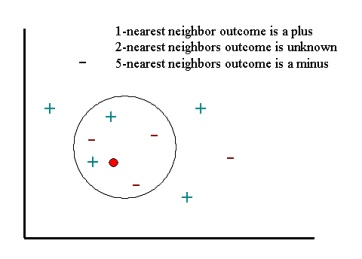
\includegraphics[width=3.0in]{figs/knn.jpg}
        \caption{Concept of $k$-NN.}
        \label{fig:bg:knn}
    \end{center}
\end{figure*}

\subsection{Na\"ive Bayes}
\subsection{Decision Tree}
\subsection{Neural Network}

\section{Data Stream Classification}
Traditional data mining algorithms work in a memory bounded environment and requires multiple scan of the training data. In stream environment, one of the major assumptions is that new data samples are introduced in the system with such a high rate that repetitive analysis becomes infeasible. Thus, for stream classification, algorithms should be able to look into a instance only once and decide upon that. A bounded memory buffer can be used to facilitate some level of repetition. However, which instances are to remember and which are to forget would then become a decision choice. An alternate choice is to maintain sufficient statistics to have a representation of the data. The process of deletion or summarization of instances, however, means that some information are being lost over the time.

In this section, these challenges are first discussed in details. Then it presents the basis of some of the concepts arisen to handle these challenges. Finally, before moving onto the ensemble leaning, it discusses current state-of-the-art algorithms for stream mining.

\subsection{Challenges}
Challenges posed by the streaming environment can be categorized into two groups: (i) relating to runtime and memory requirements and (ii) relating to underlying concept identification. Speed of incoming data, unbounded memory requirement, single-pass learning fall into the first category. On the other hand, lack of labeled data, concept drifting, evolution and recurrence are examples of latter category.

\paragraph{Speed of data arrival}
As mentioned before, it is an inherent characteristic of data streams that it arrives with a high speed. The algorithm should be able to adapt to the high speed nature of streaming information. The rate of building the classifier model should be higher than the data rate. This gives a very limited amount of available time for classification as compared to the traditional batch classification models.

\paragraph{Memory requirements:}
To apply traditional batched approaches in streaming data, an unbounded memory would be needed. This challenge has been addressed using load shedding, sampling, aggregation, etc. Rather than storing all the instances, algorithms store a subset of the data set or some statistical values or a combination of both which represents the data seen thus far. New instances can be classified only by looking into these stored information. 

\paragraph{Single-pass learning:}
The premise of this requirement is two-fold. First, as mentioned above, data would not be available in the memory after a short period of time due to the volume of data. Secondly, even if the data remain available, running a batched-like approach for millions of data points would highly increase the running time of the algorithm. To attain faster processing time with limited storage, algorithm should access the data stream only once, or a small number of times. Mining models must posses the capability to learn the underlying nature of data in a single pass over the data.

\paragraph{Lack of labeled data:}
Unlike most data sets or settings of batched approaches, steam mining data sets are often poorly labeled. A large number of experimentations are done with generated data set where the data generation process can easily be controlled to have proper labeling. However, in data set collected from real world are often lack this. For example, to setup a supervised learning experimentation using a data set collected from social media, e.g. Twitter, data needs to be first categorized by human intervention. Manual labeling of such data is often costly, both in terms of resources and time. In practice, only a small fraction of data is labeled by human experts or automated scripts. A stream classification algorithm is thus required to be able to predict after observing a small number of instances, i.e. to be ready to predict anytime.

\begin{figure*}[htbp] 
    \begin{center}
        \begin{tabular}{cc}
            \resizebox{60mm}{!}{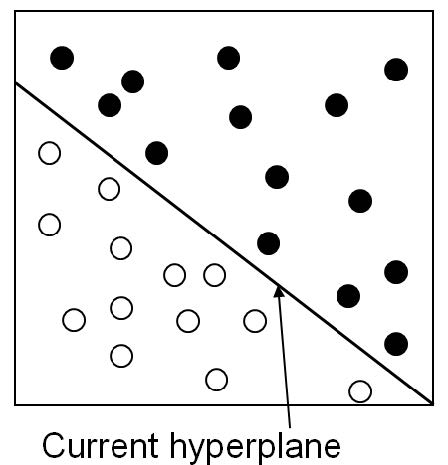
\includegraphics{figs/condrift-a.jpg}} &
            \resizebox{60mm}{!}{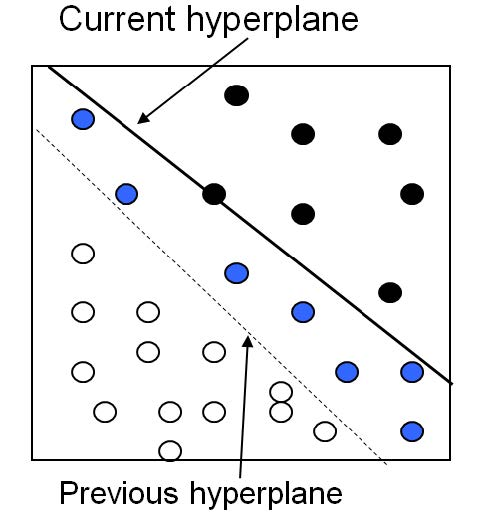
\includegraphics{figs/condrift-b.jpg}} \\
            \scriptsize{(a)\hspace{0mm}} & \scriptsize{(b)}    
        \end{tabular}
    \caption{Concept drift in data streams.}
    \label{fig:bg:condrift}
    \end{center}
\end{figure*}
\paragraph{Concept drift:}
Concept drift is a statistical property of data streams where the target variable drifts away from the model that is trying to predict it. In other words the underlying data distribution is changing over time. As a result accuracy of the classifier model decreases over time. For example, buying pattern of the customers in a store changes over time, mostly due to the seasonality. Electrical and mechanical devices wear off over time, producing shifted result which would cause drift in the observing data. Learning models should adapt to these changes quickly and accurately. Let us consider the example in Figure~\ref{fig:bg:condrift}. As a new chunk arrives (Figure~\ref{fig:bg:condrift}a), a new classifier is learned. The decision boundary is denoted by the straight line. The positive examples are represented by unfilled circles while the negative examples are represented by filled circles. With time the concept of some of the examples may change. As shown in Figure~\ref{fig:bg:condrift}b, due to concept drift some negative examples may have become positive. So, the previous decision boundary has become outdated and a new model has to be learned.

One challenge posed here is to differentiate the noise in data and the actual shift of the concept. Often in streaming environment data contains the both. 

\begin{figure*}[htbp]
    \begin{center}
        \begin{tabular}{cc}
            \resizebox{60mm}{!}{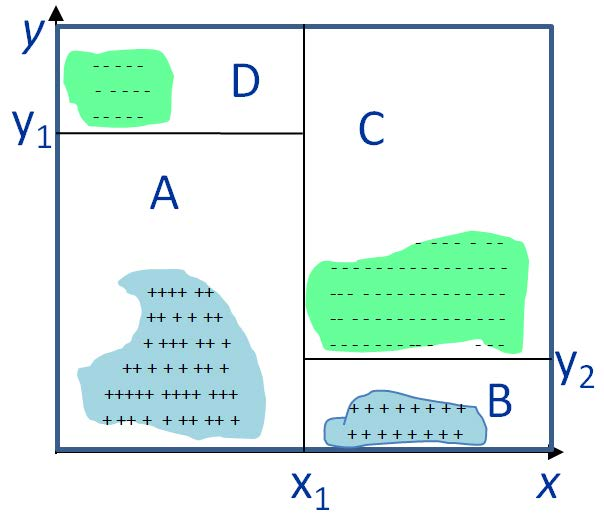
\includegraphics{figs/conevol-a.jpg}} &
            \resizebox{60mm}{!}{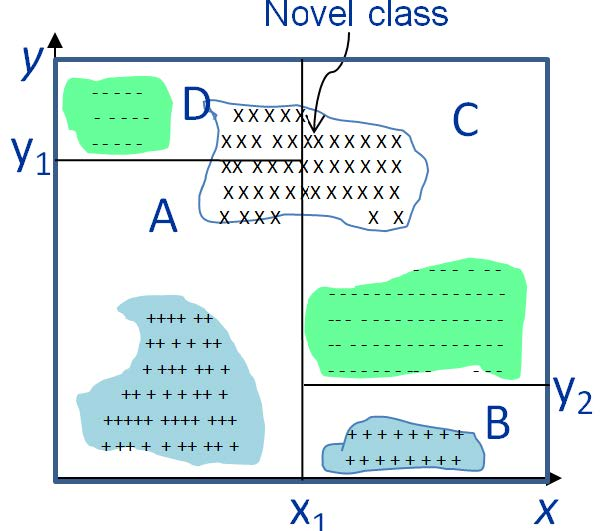
\includegraphics{figs/conevol-b.jpg}} \\
            \scriptsize{(a)\hspace{0mm}} & \scriptsize{(b)}    
        \end{tabular}
        \caption{Concept evolution in data streams.}
        \label{fig:bg:dataevol}
    \end{center}
\end{figure*}
\paragraph{Concept evolution:}
Concept evolution is referred to the emergence of a new class or a set of classes in stream data as the time flows. Twitter stream is an ideal example where concept evolution is very easily identifiable. Twitter reacts, seemingly, very fast upon important news around the globe. Looking into the different hash tag usages in such social media currently trending topics can be identified. To present a clearer picture let's consider following example in Figure~\ref{fig:bg:dataevol}. At certain point of time four classes and their corresponding decision boundaries are shown in the Figure~ (\ref{fig:bg:dataevol}a). With the more incoming data a novel class emerges, and for that decision boundaries need updating. Emergence of new class can affect any number of decision boundary/ rule, from one to all.

Concept evolution is also prone to noise. Furthermore, clear distinction between drift and evolution might not always be possible, partially due the lack of unlabeled data.

\paragraph{Class recurrence:}
Class recurrence is a special case of concept drift and evolution. A this case, the model forgets a class due the drift, however, later the class reappears (evolution) from the stream. Seasonality could be one cause of this situation. A intrusion in network traffic may reappear after a long time. Forgetting the earlier intrusions are not desired in such case. A fast recognition of the previously seen classes are desired in mining streams.

Following sections discuss the potential solutions to these challenges. First, how to address the limited resources and then the change detection schemes.

\subsection{Maintaining Sufficient Statistics}
In statistical evaluation, a statistic is sufficient for a family of probability distributions if the sample from which it is calculated gives no additional information than does the statistic, as to which of those probability distributions is that of the population from which the sample was taken~\cite{fisher22:suffstat}. Mathematically, given a set  $\mathbf{X}$ of independent identically distributed data conditioned on an unknown parameter $\theta$, a sufficient statistic is a function $T(\mathbf{X})$ whose value contains all the information needed to compute any estimate of the parameter (e.g. a maximum likelihood estimate). Due to the factorization theorem (see below), for a sufficient statistic $T(\mathbf{X})$, the joint distribution can be written as $ p(\mathbf{X}) = h(\mathbf{X}) g(\theta, T(\mathbf{X}))$. From this factorization, it can easily be seen that the maximum likelihood estimate of $\theta$ will interact with $\mathbf{X}$ only through $T(\mathbf{X})$. Typically, the sufficient statistic is a set of function or random variables of the data.

\subsubsection{Bounds of Random Variable}
A random variable is a variable that can take a set or range of values, each with an associated probability, and are subjected to change due to the alteration or randomness of the data. Random variables are of two types: (i) discrete, and (ii) continuous. Discrete random variable take a set of possible values (e.g. outcome of coin flipping), but a continuous random variable can take any value within a range (e.g. age of people in a randomly sampled group).

A function that is used to estimating a random variable is called an estimator. Estimator function is dependent on the observable sample data, and used for estimating unknown population within an interval with certain degree of confidence. For an interval of the true value of the parameter associates with a confidence of $1 - \delta$, interval can be defined as follows:

\begin{itemize}    
    \item Absolute approximation: $\bar{X} - \epsilon \le \mu \le \bar{X} + \epsilon$, where $\epsilon$ is the absolute error.
    \item Relative approximation: $(1 - \delta)\bar{X} \le \mu \le (1 + \delta)\bar{X}$, where  is the relative error.
\end{itemize}

where $\mu$ and $\bar{X}$ represent actual and estimated mean. There are a number of theorems that provide bounds on the estimation, Chebyshev [!], Chernoff~[!], Hoeffding~\cite{hoeffding63:bound}, etc. are few of them.

\begin{theorem}[Chebyshev]
\label{(thm:chebyshev)}
    Let $X$ be a random variable with standard deviation $\sigma$, the probability that the outcome of $X$ is no less than $k\sigma$ away from its mean is no more that $1/k^2$:
    $$
        P(|X-\mu| \le k\sigma) \le \frac{1}{k^2}
    $$
    In other words, it states that no more that $1/4$ of the values are more than $2$ standard deviation away, no more than $1/9$ are more than $3$ standard deviation away, and so on.
\end{theorem}

\begin{theorem}[Chernoff Bound]
\label{(thm:chernoff)}
    Let $X_1,X_2,\dots, X_n$ be independent random variables from Bernoulli experiments. Assuming that $P(X_i = 1) = p_i$. Let $X_s = P_n \sum_{i=1}{n} X_i$ be a random variable with expected value $\mu_s = P \sum_{i=1} np_i$. Then for any $\delta > 0$:
    $$
        P[X_s > (1+\delta) \mu_s] \le (\frac{e^\delta}{(1 + \delta)^{1 +\delta}} )  ^{\mu_s}
    $$
    and the absolute error is:
    $$
        \epsilon \le \sqrt{\frac{3 \bar{\mu}}{n} \ln (2/\delta)}
    $$
\end{theorem}

\begin{theorem}[Hoeffding Bound]
\label{(thm:hoeffding)}
    Let $X_1,X_2,\dots, X_n$ be independent random variables. Assuming that each $x_i$ is bounded, that is $P(X_i \in R = [a_i, b_i]) = 1$. Let $S = 1/n \sum_{i=1}{n} X_i$ whose expected value is $E[S]$. Then, for any $\epsilon > 0$:
    $$
        P[S - E[S] > \epsilon] \le e^{ \frac{2 n^2 \epsilon^2}{R^2} }
    $$
    and the absolute error is:
    $$
        \epsilon \le \sqrt{\frac{R^2 \ln(2/\delta)}{2n}}
    $$
\end{theorem}

Chernoff and Hoeffding bounds are independent of the underlying distribution of examples. They are more restrictive or conservative, and requires more observations as compared to the distribution dependent bounds. Chernoff bound is multiplicative and Hoeffding is additive. They are expressed as relative and absolute approximation, respectively.

These methods only take a finite number of values or a range. One of the well-known methods supports infinity is Poisson process. A random variable $x$ is Poisson random variable with parameter $\lambda$ if $x$ takes values $0,1,2, \dots, \infty$ with:
    $$
        p_k = P(x=k) = e^{-\lambda} \frac{\lambda^k}{k!}
    $$
    where, $\lambda$ is both mean and variance, i.e. $E(X) = Var(X) = \lambda$
    
\subsubsection{Maintaining Simple Statistics}

\subsection{Change Detection}
\subsection{Na\"ive Bayes Adaptation}
\subsection{Very Fast Decision Tree}

\section{Ensemble Learning}
Ensemble learning is a commonly used tool for building prediction models from data streams, due to
its intrinsic merits of handling large volumes stream data. Different from traditional incremental and
online learning approaches that merely rely on a single model [11, 38], ensemble learning employs a
divide-and-conquer approach to first split the continuous data streams into small data chunks, and
then build light-weight base classifiers from the small chunks. At the final stage, all base classifiers are
combined together for prediction. By doing so, an ensemble model can enjoy a number of advantages,
such as scaling up to large volumes of stream data, adapting quickly to new concepts, achieving lower
variances than a single model, and easily to be parallelized.
Ensemble classifiers on data streams provide a generic framework for handling massive volume data
streams with concept drifting. The idea of ensemble classifiers is to partition continuous data streams
into small data chunks, from which a number of base classifiers are built and combined together for
prediction. Two main motivations for combining classifiers are as follows:

Statistical (or worst case) motivation: It is possible to avoid the worst classifier by averaging
several classifiers. It was confirmed theoretically by Fumera and Roli in [39]. This simple
combination was demonstrated to be efficient in many applications. There is no guarantee,however, the combination will perform better than the best classifier.

Representational (or best case) motivation: Under particular situations, fusion of multiple
classifiers can improve the performance of the best individual classifier. It happens when the
optimal classifier for a problem is outside of the considered classifier space". There are many
experimental evidences that it is possible if the classifiers in an ensemble make different errors.
This assumption has a theoretical support in some cases when linear combination is performed.



\subsection{Bagging}
\subsection{Boosting}
\subsection{ASHT}
\subsection{...}

\bibliographystyle{apalike}
\bibliography{ref}

\end{document}
